\documentclass{article}
\usepackage{amsmath}
\usepackage{amsfonts}
\usepackage{graphicx}

\title{Hola, mundo}
\author{Claudio Gonzalo Villarreal Araujo}

\begin{document}
	
	\maketitle
	
	\section{Comenzando}
	Hola, mundo. Hoy estoy aprendiendo \LaTeX. \LaTeX\ es un excelente lenguaje para producir documentos académicos. Puedo escribir matemáticas en línea, como \( a^2 + b^2 = c^2 \). También puedo darle a las ecuaciones su propia línea:
	\begin{equation}
		\gamma^2 + \theta^2 = \omega^2
	\end{equation}
	Las “ecuaciones de Maxwell” son nombradas en honor a James Clark Maxwell y son las siguientes:
	
	\begin{align}
		\vec{\nabla} \cdot \vec{E} &= \frac{\rho}{\epsilon_0} && \text{Ley de Gauss} \\
		\vec{\nabla} \cdot \vec{B} &= 0 && \text{Ley de Gauss para el magnetismo} \\
		\vec{\nabla} \times \vec{E} &= - \frac{\partial \vec{B}}{\partial t} && \text{Ley de Faraday} \\
		\vec{\nabla} \times \vec{B} &= \mu_0 \left( \epsilon_0 \frac{\partial \vec{E}}{\partial t} + \vec{J} \right) && \text{Ley de Ampere}
	\end{align}
	Las ecuaciones \(2\), \(3\), \(4\) y \(5\) son algunas de las ecuaciones más importantes en Física.
	
	\section{¿Qué hay sobre las ecuaciones matriciales?}
	
\[
\begin{pmatrix}
	a_{11} & a_{12} & \cdots & a_{1n} \\
	a_{21} & a_{22} & \cdots & a_{2n} \\
	\vdots & \vdots & \ddots & \vdots \\
	a_{n1} & a_{n2} & \cdots & a_{nn}
\end{pmatrix}
\begin{bmatrix}
	v_1 \\
	v_2 \\
	\vdots \\
	v_n
\end{bmatrix}
=
\begin{array}{cc}
	\omega_1 \\
	\omega_2 \\
	\vdots \\
	\omega_n
\end{array}
\]

\section{Tablas y Figuras}

Crear una tabla no es muy diferente de crear una matriz:

\begin{table}[h!]
	\caption{Mi primera tabla.}
	\centering
	\begin{tabular}{|l||c|c|c|}
		\hline
		\textbf{\(x\)} & 1 & 2 & 3 \\
		\hline
		\(f(x)\) & 4 & 8 & 12 \\
		f(x) & 4 & 8 & 12 \\
		\hline
	\end{tabular}
	
\end{table}

\begin{figure}[h!]
	\centering
		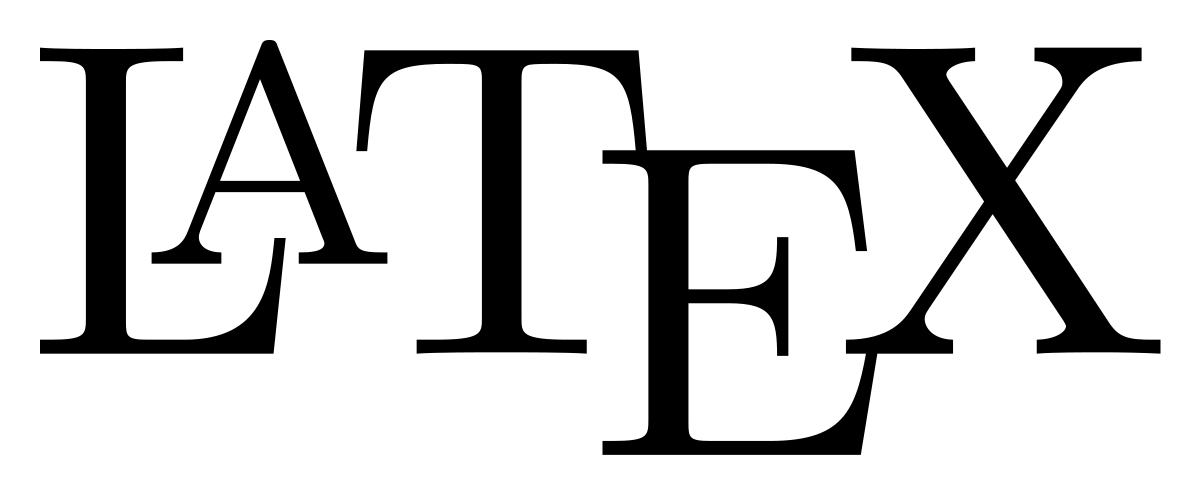
\includegraphics[width=0.5\textwidth]{imagen.png}
	\caption{Cualquier imagen.}
\end{figure}

\end{document}